\chapter{Wstęp i cel pracy} 

Laserowy tomograf komputerowy to innowacyjne urządzenie opracowywane i udoskonalane w ramach szeregu projektów naukowych poświęconych dozymetrii wielowymiarowej wysokiej rozdzielczości na Wydziale Fizyki Technicznej i Matematyki Stosowanej PG. W \cite{algo} przedstawiono w postaci schematu blokowego proces pozyskiwania oraz przetwarzania obrazów w celach radioterapeutycznych. Dodanie do niego symulacji LCT jeszcze bardziej rozbuduje istniejący algorytm postępowania, ale umożliwi porównanie rozkładu dawki w przestrzeni trójwymiarowej otrzymanej w ramach symulacji z teoretycznymi oczekiwaniami wyliczonymi przez odpowiedni algorytm (bazujące na wokselach, jeżeli do diagnostyki zastosowano metodę SPECT/CT, to metody niesztywne rejestracji obrazów przyczyniają się do poprawy rozdzielczości \cite{image}). Docelowo rozwiązanie to ma zostać wykorzystane m.in.: przez oddziały radiologiczne w szpitalach w celach dozymetrycznych, konkretnie do symulacji przygotowanych przez fizyków medycznych planów leczenia nowotworów. 

Do najważniejszych elementów LCT można zaliczyć: laser, zwierciadło zamontowane na silniku krokowym (lub też silniku rezonansowym), akwarium (w którym umieszcza się fantom polimerowo-żelowy) i detektor promieniowania optycznego. Sama wiązka po odbiciu od zwierciadła jest modyfikowana specjalnymi soczewkami. Wykorzystywany laserowy tomograf komputerowy został bardziej szczegółowo opisany w \cite{Mar}.

\begin{figure}[H]
    \centering
    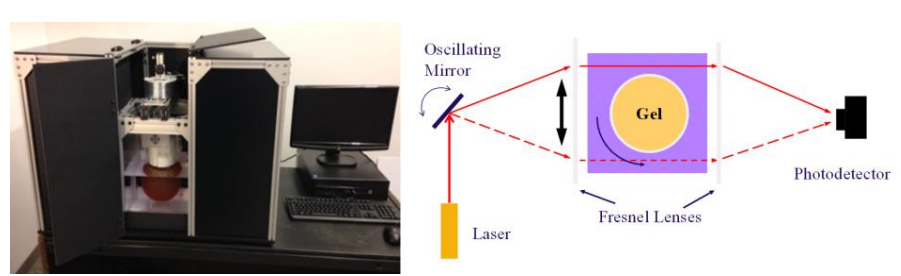
\includegraphics[width=\textwidth]{pictures/LCT_diagram.png}
    \caption{Wygląd oraz schemat tomografu \cite{Mar}}
    \label{fig:LCT}
\end{figure}

Omawiane urządzenie ma przyczynić się do wzrostu bezpieczeństwa i skuteczności radioterapii, jak również przyspieszyć i zoptymalizować pracę samego fizyka medycznego. Z tego powodu, pożądana jest możliwie jak największa automatyzacja działania tomografu. Jednym z aspektów do usamodzielnienia jest diagnostyka działania LCT. Opracowany aparat jest prototypem zbudowanym ręcznie. Trzeba więc w analizie błędów uwzględnić potencjalny czynnik ludzki.

Przy leczeniu wykorzystującym teleradioterapię, niezwykle istotna jest dokładność, jak i precyzja, z jaką deponowana jest dawka promieniowania w guzie nowotworowym oraz jego otoczeniu. W miarę możliwości należy unikać niepotrzebnego narażania tkanek zdrowych oraz narządów krytycznych na uszkodzenia wywołane promieniowaniem. Dlatego też przy symulacjach należy zadbać o możliwie najwierniejsze odzwierciedlenie docelowej operacji, niwelując przy tym błędy mogące wynikać z samego działania urządzenia. W tym celu potrzebna jest dodatkowa aparatura, która umożliwi szybką i sprawną analizę działania samego LCT.

\newpage

Szczególną uwagę trzeba poświęcić silnikowi krokowemu i przymocowanemu do niego zwierciadełku. Kształt zwierciadła (kołowy) pozwala na łatwiejsze zachowanie symetrii. Jednakże, przez potencjalne nieidealne umieszczenie zwierciadła na elemencie obrotowym mogą powstać asymetryczne momenty bezwładności, które będą bezpośrednio wpływać na prędkość obrotową samego elementu (na charakterystyce zmiany położenia objawiłoby się to w postaci niesymetrycznej sinusoidy). Przykładowy silnik krokowy z Amazona przedstawia rysunek 1.2. Kątownik jest przymocowany do silnika, po jednej stronie ma przymocowane zwierciadło, a po drugiej moduł SEN0142 (rozdział 3.3).

\begin{figure}[H]
    \centering
    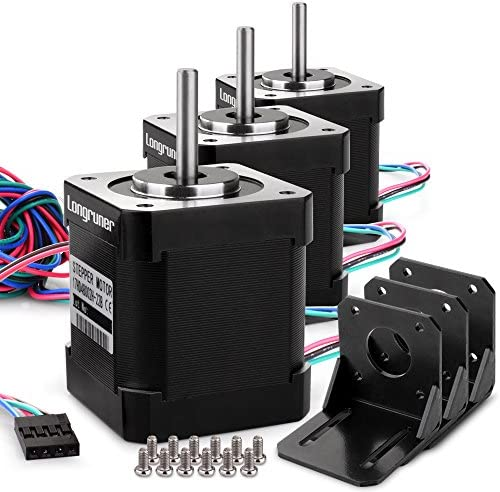
\includegraphics[width=0.6\textwidth]{pictures/silnik.jpg}
    \caption{Przykładowy silnik krokowy}
    \label{fig:silnik}
\end{figure}

Celem pracy jest zaprojektowanie i zbudowanie czujnika wraz z oprogramowaniem, umożliwiającego zautomatyzowany pomiar zmian położenia elementu obrotowego silnika krokowego. Pozwoli to na zaobserwowanie potencjalnych nieprawidłowości w zmianach kątowych poruszającego się zwierciadła, dzięki czemu możliwa będzie szybka reakcja i korekta elementu. Praca ma skupić się na:

\begin{enumerate}
    \item analizie nowych rozwiązań zagadnienia,
    \item zaimplementowaniu wybranego rozwiązania,
    \item testowaniu i udoskonaleniu stworzonego programu.
\end{enumerate}